\chapter{Projektorganisation}
	\documentSubPartEntry{Projektorganisation}

	\section{Projektteam}
	Für das Projekt verantwortlich sind Laurin Murer und Tobias Blaser.
	Sie sind beide Informatik-Studenten an der HSR und schliessen das Studium im Winter 2014/2015 ab.
	\begin{figure}[H]
		\begin{minipage}[b]{0.5\linewidth}
			
\includegraphics[width=0.5\textwidth]{projectPlan/media/img/lmurer.jpg}
			\centering
			\caption{Laurin Murer}
			\label{fig:laurinmurer}
		\end{minipage}
		\begin{minipage}[b]{0.5\linewidth}
			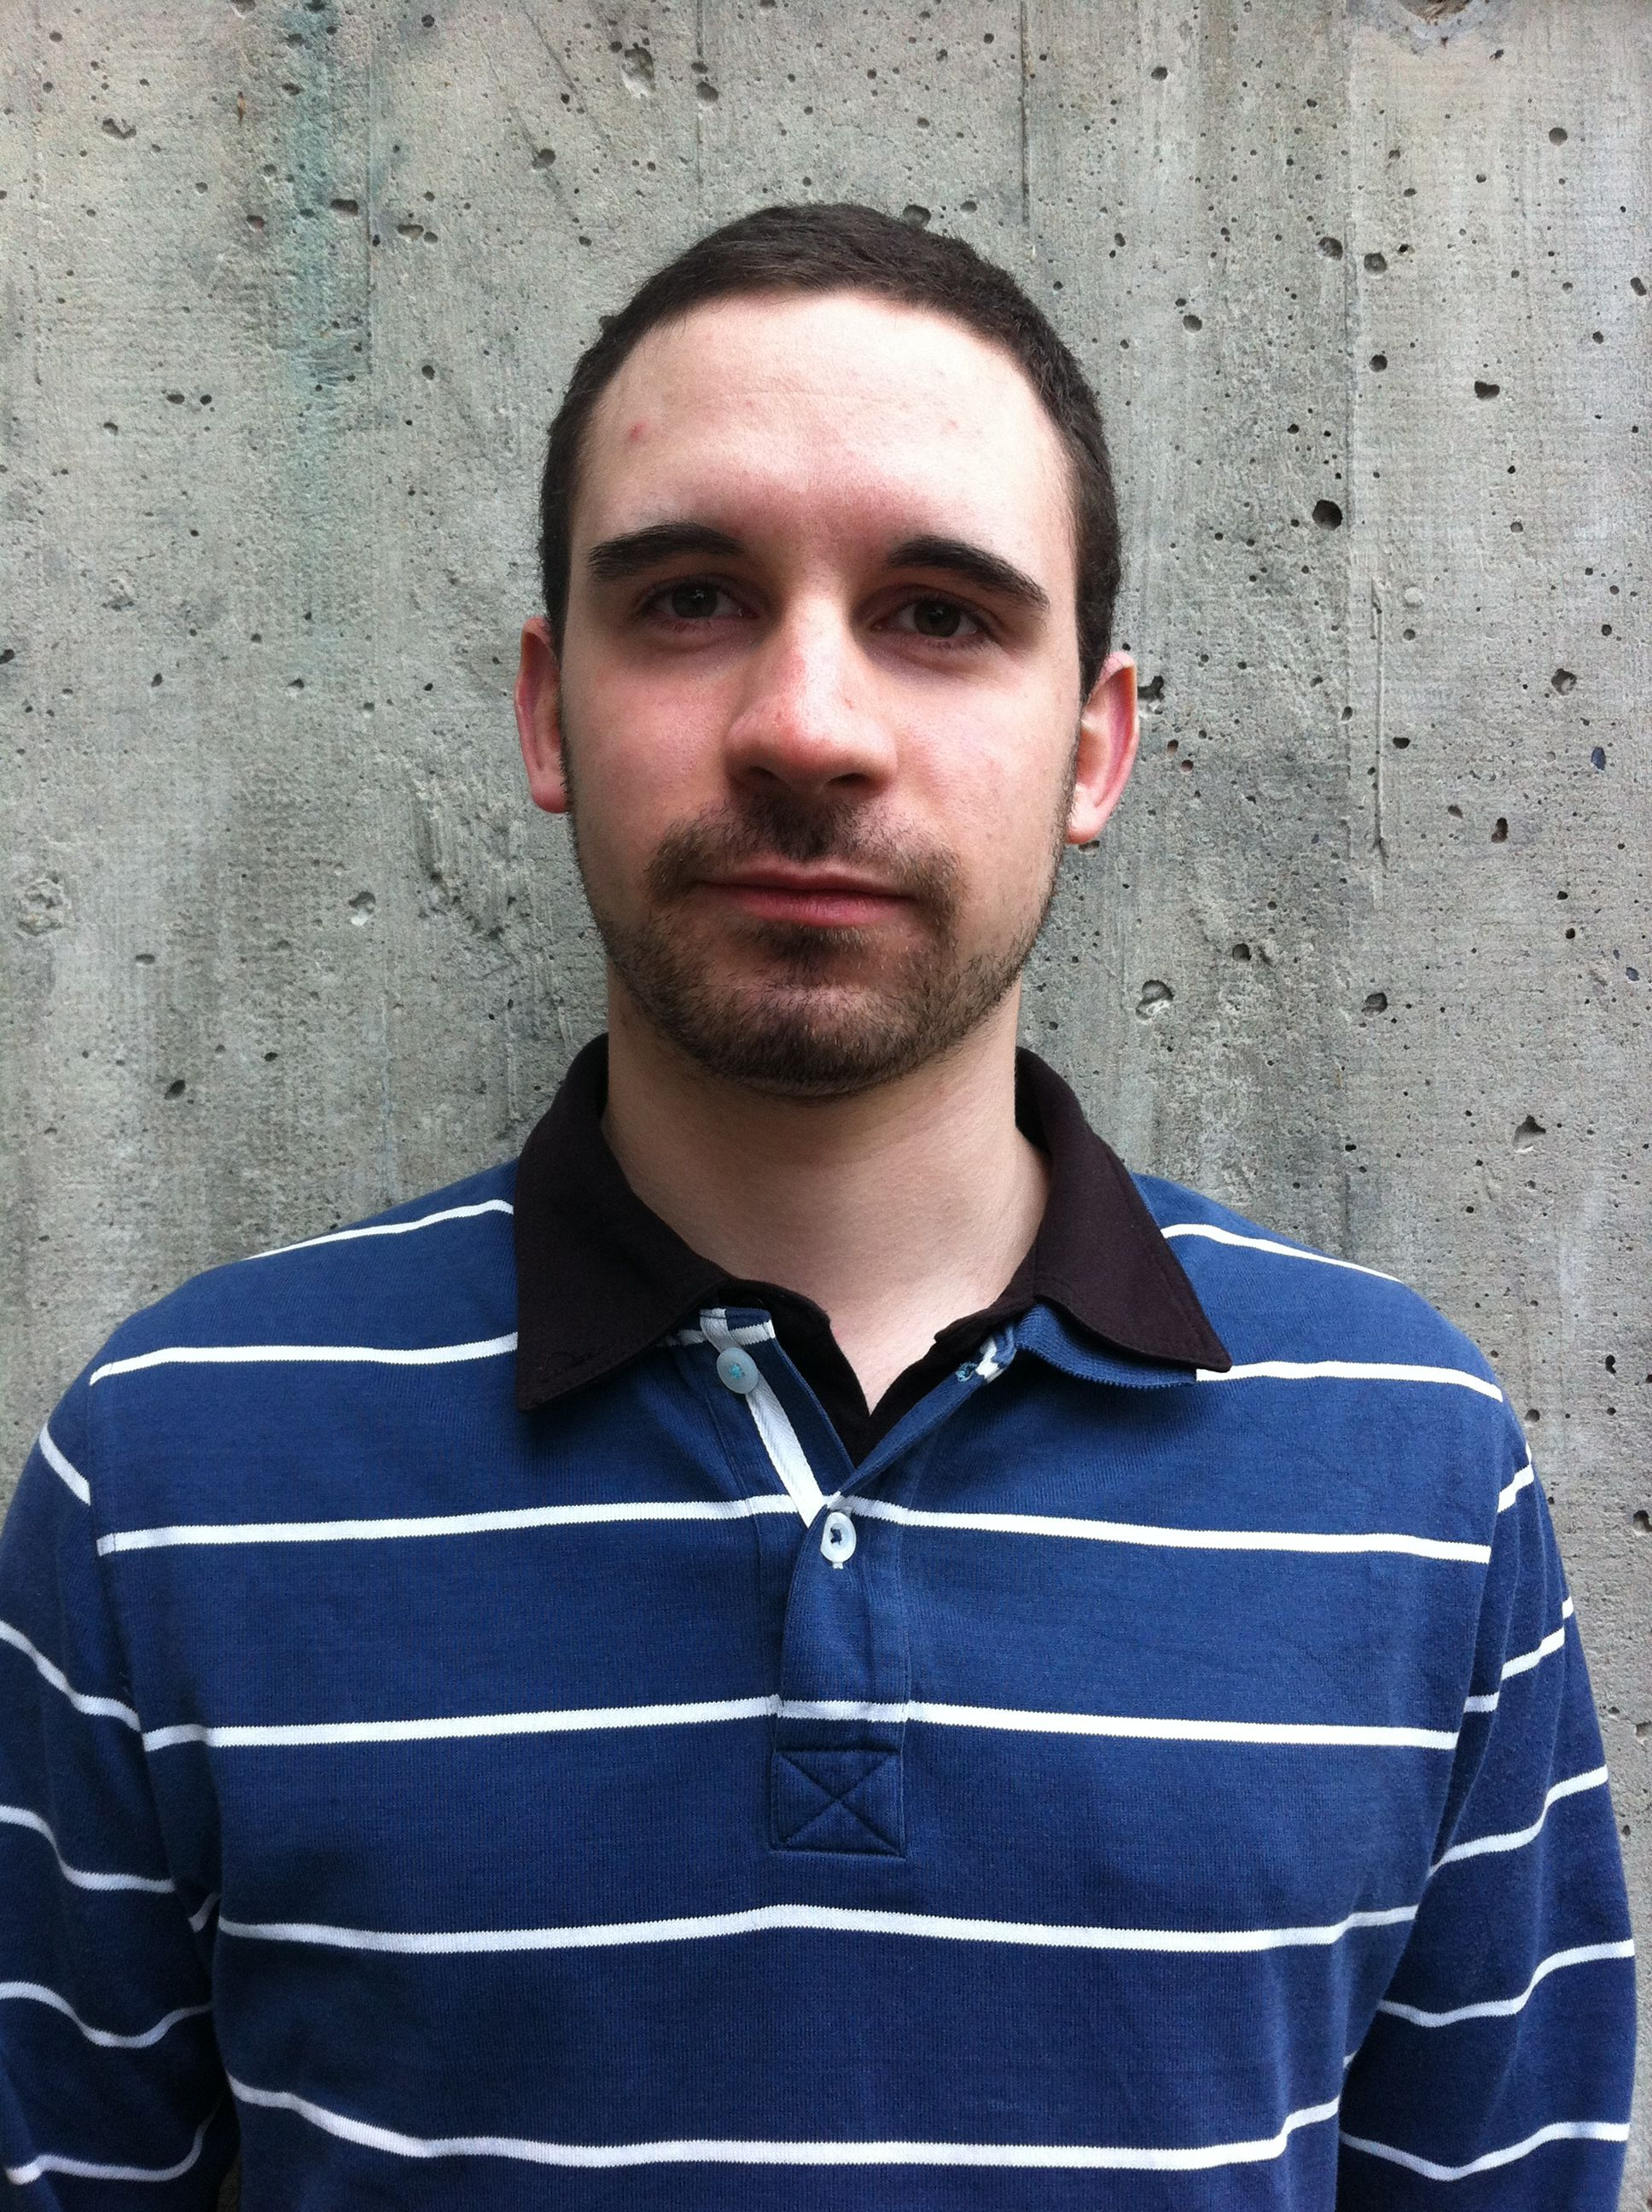
\includegraphics[width=0.5\textwidth]{projectPlan/media/img/tblaser.jpg}
			\centering
			\caption{Tobias Blaser}
			\label{fig:tobiasblaser}
		\end{minipage}
	\end{figure}

	\section{Projektbegleitung}
	Der Betreuer des Projekts ist Prof. Dr. Olaf Zimmermann.
	Er ist Dozent an der HSR mit Schwerpunkt Software Architecture, Enterprise SOA und Cloud \cite{zimmermann_ifs_2014}.
	\begin{figure}[H]
		\begin{minipage}[b]{0.5\linewidth}
			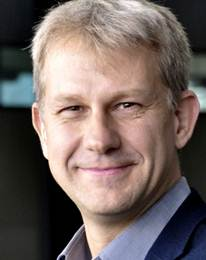
\includegraphics[width=0.5\textwidth]{projectPlan/media/img/ozimmermann.jpg}
			\centering
			\caption{\teacher}
			\label{fig:olafzimmermann}
		\end{minipage}
	\end{figure}
	Er betreut die Semesterarbeit und begleitet das Team durch regelmässige Meetings.
	Für das Projekt vertritt er ausserdem die Kundengruppe.


	\section{Projekt- und Qualitätsmanagement}
		Zur Verwaltung des Projektes hat das Projektteam ein Jira eingesetzt,
		wobei Jira-Versions zur Meilensteinplanung zum Einsatz kamen.
		
		\begin{figure}[H]
			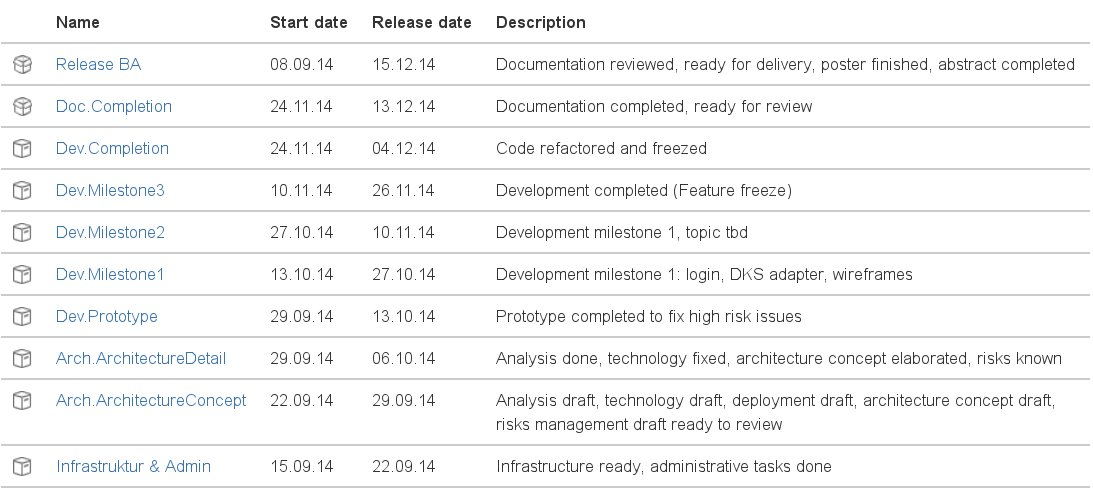
\includegraphics[width=\textwidth]{projectPlan/media/img/jiraVersions.jpg}
			\centering
			\caption{Jira Versions/Meilensteine}
			\label{fig:jiraVersions}
		\end{figure}
		
		Im Abschnitt~\ref{cap:projectmanagement} auf Seite \pageref{cap:projectmanagement} wird das Projekt- und Qualitätsmanagement mit Jira und Git detailliert erläutert.
	
